\documentclass[10pt]{article}
\usepackage[UTF8]{ctex}
\usepackage[a4paper,left=15mm,right=15mm,top=16mm,bottom=19mm]{geometry}
\usepackage{xeCJKfntef}
\usepackage{fontspec}
\usepackage{amsmath,amsfonts,amssymb}
\usepackage{tikz}
\usepackage{pifont}
\usepackage{subfigure}
\usepackage{float}
\usepackage{caption}
\usetikzlibrary{arrows.meta}
\renewcommand{\figurename}{}
\renewcommand{\thesubfigure}{}
\makeatletter \renewcommand{\@thesubfigure}{\thesubfigure \space}
\renewcommand{\p@subfigure}{} \makeatother
\setmainfont{Times New Roman}
\newcommand{\circnum}[1]{\ding{\numexpr171+#1\relax}}
\newcommand{\addspace}{\hspace*{\fill} \\ \hspace*{\fill} \\\hspace*{\fill}\\ \hspace*{\fill} \\\hspace*{\fill}\\ \hspace*{\fill} \\\hspace*{\fill}}
\newcommand{\complitingline}{\_\_\_\_\_\_\_\_\_}
\newcommand{\textdot}[1]{{\heiti \CJKunderdot{#1}}}
\usepackage{lastpage}
\usepackage{fancyhdr}
\pagestyle{fancy}
\cfoot{数学试卷~~~第\thepage 页(共 \pageref{LastPage} 页)}
\renewcommand{\headrulewidth}{0mm}
%选择题盒子,1行4选项
\newcommand{\onp} [4] { \\
    \begin{tabular} {*{4}{@{}p{3.5cm}}}
        A.~#1 & B.~#2 & C.~#3 & D.~#4
    \end{tabular}
}
%选择题盒子,1行2选项
\newcommand{\twp} [4] { \\
    \begin{tabular} {*{2}{@{}p{7cm}}}
        A.~#1 & B.~#2
    \end{tabular} \\
    \begin{tabular} {*{2}{@{}p{7cm}}}
        C.~#3 & D.~#4
    \end{tabular}
}
%选择题盒子,1行1选项
\newcommand{\fop} [4] { \\
    A.~#1 \\
    B.~#2 \\
    C.~#3 \\
    D.~#4
}
%图片盒子 参数1为路径 2为大小
\newcommand{\smallpicture}[2]{\includegraphics[scale = #2]{#1}}
\usepackage{graphicx}  %插图包
\usepackage{paralist}  %序号包
%定位器 参数1、2为横纵坐标 3为插入盒子
\newcommand{\pbox} [3] {
    \unitlength=1mm
    \begin{picture} (0, 0)
        \put (#1, #2) {#3}
    \end{picture}
}
\begin{document}
\section*{\centering 第二十一章~~~一元二次方程}
\centerline{时间:2小时 \ \ \ \ 满分:120分}
\section*{\normalsize 一、选择题(每小题3分,共30分)}
\begin{enumerate}\setcounter{enumi}{0}
    \item 关于$x$的一元二次方程$bx^{2} + 18x - 4c = 4$的一次项和常数项系数分别为(~~~~~~~)。
    \onp{$18$,$-4c$}{$b$,$4c+4$}{$18$,$-4c-4$}{$18$,$-4c$}
    \item 下列关于$x$的方程中,是一元二次方程的是(~~~~~~~)。
    \twp{$4x^{2} + x = (2x + 1)^{2}$}{$\frac{x^{3} + 5x^{2} + 18x}{5x} = 0$}{$( x^{2} + x )^{0} - 1 = 0$}{$- x^2 + 3 = 1$}
    \item 已知关于$x$的一元二次方程$- x^{2} + 2ax = 3b$,则(~~~~~~~)。
    \twp{$x_{1} + x_{2} = - 2a$}{$x_{1}x_{2} = 3b$}{$x_{1} - x_{2} = 2\sqrt{a^{2} - 3b}$}{$x_{1} + 2x_{2} = 2a + b$}
    \item 若关于$x$的方程$ax^{2} + bx + c = 0$有解,则下列说法正确的是(~~~~~~~)。
    \twp{方程有两个实数根}{$c = 0$时,$x$必有一解为$0$}{当$a > 0$时,方程有两个相等实数根}{$b$不可能为$0$}
    \item 若关于$x$的一元二次方程有两个解$x_{1} = 1$,$x_{2} = 2$,则这个方程可能是(~~~~~~~)。
    \twp{$x^{2} + 3x = 2$}{$x^{2} - 3x + 2 = 0$}{$x^{2} - 2x + 3 = 0$}{$x^{2} + 3x = - 2$}
    \item 如图,在平行四边形$ABCD$中,$AD=6$,$BD=\sqrt{205}$,连对角线$AB$,有$AB \bot CB$,延长$CB$至$F$,使$CB=FB$,在线段$AB$上取点$E$,连$EF$,使$EF=2AE$,则$BE$的长度为(~~~~~~~)。
    \onp{$5$}{$8$}{$10$}{$6$}
    \item 已知理想情况下物体在做自由落体运动时,下落距离$s$与时间$t$满足以下关系:$s = 4.9t^{2}$,若一个物体下落了$181.8$m,则下列等式正确的是(~~~~~~~)。
    \twp{$4.9s = {181.8}^{2}$}{$4.9t^{2} = \frac{181.8}{4.9}$}{$t = \sqrt{\frac{181.8}{4.9}}$}{$\sqrt{181.8} = t + 4.9$}
    \item 如图,为一种轻质的老式秤。某次称量时,称量的物品和秤盘的总质量为$800$g,秤砣到手拉环的距离为$s$cm时,刚好平衡。若秤盘到手拉环的距离为$5$cm,秤砣质量为$m$g,且$m$和$s$满足$m=8s+40$,则$s$的值为(~~~~~~~)。
    \onp{$30$}{$25$}{$20$}{$55$}

    \item 计算$(\frac{1+\sqrt{5}}{2})^8+(\frac{1-\sqrt{5}}{2})^8$的值为(~~~~~~~)。
    \onp{$5$}{$47$}{$34$}{$58$}
    \item 已知在$\Delta ABC$中,$AB = AC$,$AE = EF = FC = CB$,则$\angle A$的大小为(~~~~~~~)。
    \onp{$15^{\circ}$}{$20^{\circ}$}{$22.5^{\circ}$}{$30^{\circ}$}
    \begin{figure}[!ht]
        \centering
        \subfigure[(第6题)]{
            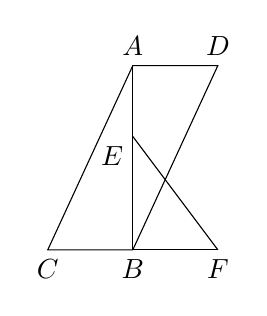
\begin{tikzpicture}[scale=0.18]
                \node[above] at (0,13) {$A$};
                \node[below] at (0,0) {$B$};
                \node[below] at (-6,0) {$C$};
                \node[below] at (6,0) {$F$};
                \node[above] at (6,13) {$D$};
                \node[below left] at (0,8) {$E$};
                \draw (-6,0)--(0,13)--(6,13)--(0,0)--cycle;
                \draw (0,13)--(0,0);
                \draw (0,0)--(6,0);
                \draw (0,8)--(6,0);
            \end{tikzpicture}
        }
        \qquad\qquad\qquad
        \subfigure[(第8题)]{
            \smallpicture{./images/T8.png}{1}
        }
        \qquad\qquad\qquad
        \subfigure[(第10题)]{
            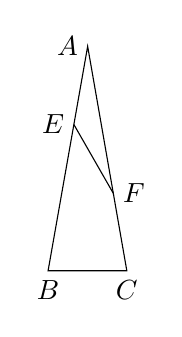
\begin{tikzpicture}[scale=0.25]
                \node[left] at (2.01,11.40) {$A$};
                \node[below] at (0,0) {$B$};
                \node[below] at (4,0) {$C$};
                \node[left] at (1.31,7.43) {$E$};
                \node[right] at (3.31,3.94) {$F$};
                \draw (2.01,11.40)--(0,0)--(4,0)--cycle;
                \draw (1.31,7.43)--(3.31,3.94);
            \end{tikzpicture}
        }
    \end{figure}
\end{enumerate}
\section*{\normalsize 二、填空题(每小题3分,共18分)}
\begin{enumerate}\setcounter{enumi}{10}
    \item 在一元二次方程$ax^{2} + 2ax + b = 0$中,一次项系数为\complitingline{},常数项系数为\complitingline{},两根之和为\complitingline{}。
    \item 已知一元二次方程中$x^{2} - ( m^{2} - 3 )x + m = 0$,有$x_{1} + x_{2} = 2$,则$m =$\complitingline{}。
    \item 若方程$x^{2} + 2x - 3 = 0$与$x^{2} + bx + 3 = 0$有一个公共解,则$b =$\complitingline{}。
    \item 已知两实数$m$、$n$满足$m^2-3m+1=0$,$n^2-3n+1=0$,且$m \neq n$,则代数式$\sqrt{\frac{m}{n}}+\sqrt{\frac{n}{m}}$的值为\complitingline{}。
    \item 已知两实数$m$,$n$满足$m^2+3m-9=0$,$9n^2-3n-1=0$,且$mn \neq 1$,则$\frac{mn+n+mn^{2}}{n^{2}}$的值为\complitingline{}。
    \item 设$a_{1} = 1 + \frac{1}{1^{2}} + \frac{1}{2^{2}} $,$ a_{2} = 1 + \frac{1}{2^{2}} + \frac{1}{3^{2}}   $,......,$a_{n} = 1 + \frac{1}{n^{2}} + \frac{1}{(n + 1)^{2}}$,其中$n$为正整数,则$\sqrt{a_{1}}$+$\sqrt{a_{2}}$+$\sqrt{a_{3}}$+......+$\sqrt{a_{2020}}$的值为\complitingline{}。
\end{enumerate}
\section*{\normalsize 三、解答题(共8题、72分,每小题应写出文字说明、解答过程或演算步骤)}
\begin{enumerate}\setcounter{enumi}{16}
    \item 用因式分解法解下列方程。
    \begin{compactenum}[(1)]
        \item $x^2-6x+8=0$
        \item $(2x+3)^2=x^2$
        \item $x^2-2ax-5x+a^2+5a+6=0$
        \item $ax^2-3a^2x-x+3a=0 \ \ \ \ \ (a \neq 0)$
    \end{compactenum}
    \addspace{}
    \item 阅读材料,完成任务。\par
    ~~~~~~~我们已经知道,对于关于$x$的一元二次方程$ax^2+bx+c=0$,由韦达定理,$x_1+x_2=-\frac{b}{a}$,$x_1x_2=\frac{c}{a}$。如果用$a$、$x_1$、$x_2$来表示$b$、$c$,那么代数式$ax^2+bx+c$可以化为$ax^2-a(x_1+x_2)x+ax_1x_2$,即$a(x-x_1)(x-x_2)$,这意味着,\textdot{对于任意的二次三项式$ax^2+bx+c$,如果一元二次方程$ax^2+bx+c=0$有实根为$x_1$,$x_2$,那么原式可因式分解为$a(x-x_1)(x-x_2)$},利用这种方法,我们可以实现二次三项式在实数范围内的因式分解。
    \begin{compactenum}[(1)]
        \item 在实数范围内因式分解下面的代数式:
        \begin{compactenum}
            \item[\circnum{1}] $x^2-x-1$
            \item[\circnum{2}] $2x^2-8x+5$
            \item[\circnum{3}] $x^4-4x^3+2x^2-4x+1$
        \end{compactenum}
        \item 试说明为什么二次三项式$x^2+x+1$无法在实数范围内被因式分解。
    \end{compactenum}
    \newpage
    \item 已知两个一元二次方程$M:ax^{2} + bx + c = 0$,$N:cx^{2} + bx + a = 0$。其中$ac \neq 0$且$a \neq c$。
    \begin{compactenum}[(1)]
        \item 如果$M$有两个相等的实数根,求证:$N$也有两个相等的实数根。
        \item 如果$M$与$N$有实数根,求证:$M$有一个根与$N$两根中的一个互为倒数。
        \item 求证:如果$M$的两根符号相同,那么$N$的两根符号也相同。
    \end{compactenum}
    \addspace{}
    \item 在实数范围内解方程组$\left\{ \begin{matrix}
        (x + 1)(y + 1) = 18 \\
        x^{2}y + xy^{2} = 66 \\
        \end{matrix} \right.$。
    \addspace{}
    \item ``读书可以让人保持思想活力,让人得到智慧启发,让人滋养浩然之气''。某校为响应我市全民阅读活动,利用节假日面向社会开放学校图书馆。据统计,第一个月进馆$128$人次,进馆人次逐月增加,到第三个月末累计进馆$608$人次。
    \begin{compactenum}[(1)]
        \item 若进馆人次的月平均增长率相同,求进馆人次的月平均增长率。
        \item 若因条件限制,学校图书馆每月接纳能力不超过$1000$人次,在进馆人次的月平均增长率不变的条件下,校图书馆第几月会接纳能力不足?在不超过接纳限度内最多可接纳多少人次?
        \item 现图书馆举行活动,给每人发送活动邀请,每人转发三位好友(保证每人恰好转发$3$个没有获得书签的好友)即可获得书签一个,若每个书签$0.5$元,第一轮只有一人转发,则三轮发送后,图书馆要支出多少钱用于购买书签?
    \end{compactenum}
    \addspace{}
    \item 已知关于$x$的一元二次方程$M:x^2+(k-2)x-k^2-1=0$。
    \begin{compactenum}[(1)]
        \item 求证:$M$有不相等的两个实根,且两根一正一负。
        \item 若$M$的两个根中,一根大于$k$,一根小于$k$,求$k$的取值范围。
    \end{compactenum}
    \newpage
    \item
    \begin{compactenum}[(1)]
        \item 已知$x$为实数,求$x^2-8x+5$的最小值。
        \item 已知$x$为实数,求代数式$\frac{x^2+x+1}{x^2+1}$的取值范围。
        \item 已知$x,y$均为实数,直接写出$-3x^2+3xy+6x-y^2$的最大值。
    \end{compactenum}
    \addspace{}
    \item 如图,在平面直角坐标系中,$A$在$y$轴正半轴上,$B$、$C$为$x$轴上两动点。
    \begin{compactenum}[(1)]
        \item 如图1,$A(0,4)$,$B$从$(-5,0)$出发,$C$从$(5,0)$出发,都以每秒$t$个单位长度向$x$轴负半轴方向运动,连$AB$、$AC$。
        \begin{compactenum}
            \item[\circnum{1}] 当$\angle BAC=90^{\circ}$时,直接写出直线$AC$的解析式。
            \item[\circnum{2}] 在\circnum{1}的条件下,若$P$为线段$AC$上一点,作$PM$垂直于$x$轴于点$M$,作$PN$垂直于$y$轴于点$N$,求四边形$OMPN$面积的最大值。
        \end{compactenum}
        \item 如图2,直线$AB:y=-\sqrt{3}x+b$,$C$在$B$左侧,$E(m,n)$为射线$AB$上一点,$CD=2m$,连接$AC$,$CE$,$DE$,若$AC=6$,$DE=5$,求$CE$的取值范围。
    \end{compactenum}
    \begin{figure}[htb]
        \centering
        \subfigure[(1)]{
        \begin{tikzpicture}[>=Stealth,scale=0.65]
            \draw[->] (-6.5,0)--(6.5,0) node[below] {$x$};
            \draw[->] (0,-1)--(0,6.5) node[left] {$y$};
            \node[below right] at (0,0) {$O$};
            \node[above right] at (0,4) {$A$};
            \node[below] at (-5,0) {$B$};
            \node[below] at (5,0) {$C$};
            \draw (-5,0)--(0,4)--(5,0);
        \end{tikzpicture}
        }
        \qquad
        \subfigure[(2)]{
        \begin{tikzpicture}[>=Stealth,scale=0.65]
            \draw[->] (-4.5,0)--(4,0) node[below] {$x$};
            \draw[->] (0,-1)--(0,6.5) node[left] {$y$};
            \node[below right] at (0,0) {$O$};
            \node[left] at (0,5) {$A$};
            \node[right] at (0.5,4.13397) {$E$};
            \node[below] at (-0.4,0) {$C$};
            \node[below right] at (0.6,0) {$D$};
            \node[below] at (2.88675,0) {$B$};
            \draw (0,5)--(2.88675,0);
            \draw (0,5)--(-0.4,0);
            \draw (-0.4,0)--(0.5,4.13397);
            \draw (0.6,0)--(0.5,4.13397);
        \end{tikzpicture}}
        \caption*{(第24题)}
    \end{figure}
\end{enumerate}
\end{document}